\documentclass[10pt]{article}
\usepackage{icmlko}

\icmlmeta{IP 파운데이션 월드모델}{59}{순위는 다섯 배, 절대값은 두 배 반}{순서를 잘 가르는 것과 값을 좁히는 것은 다른 일이었다 --- 그 간극을 숫자로 적는다}

\begin{document}

\twocolumn[
\icmlheader

\begin{abstract}
노트 58은 팝업 예측 상위 20\%가 860명, 하위 20\%가 157명으로 5.5배 갈린다고
했다. 그런데 그것은 \emph{순위}다. 예측값에는 눈금이 없어 ``이 기획은 몇 명''을
말하지 못한다. 노트 26 · 32에서 세운 절차 --- 대상 도메인 몇 건을 실제로 재서
중심과 산포를 맞춘다 --- 를 여섯 도메인에서 다시 쟀다. \textbf{열두 건을 재면
절대 예측 오차가 $\times\div$2.51배다.} 같은 열두 건으로 중앙값만 쓰면
$\times\div$2.82배이므로 모델이 줄이는 몫은 11\%다. $k$를 서른까지 늘려도
2.41배로 거의 안 줄어든다 --- \textbf{눈금은 여덟에서 열둘이면 잡힌다}는
노트 32의 결론이 여섯 도메인에서 확인된다. 문제는 눈금이 아니라 잔차다.
순위 상관이 $+$0.47이면 설명되는 분산이 22\%이고 잔차 표준편차가 원래의 88\%로
남는다. \textbf{순서는 5.5배로 가르는데 값은 2.5배 안으로 못 좁힌다.}
443명이라고 예측하면 실제는 대략 180명에서 1,100명 사이다. 제품 진술을 정확히
쓰면 이렇게 된다 --- \textbf{어느 기획을 먼저 밀지 고르는 데는 쓸 수 있고,
몇 명 올지 약속하는 데는 아직 못 쓴다.}
\end{abstract}
]

\section{순위에 눈금을 붙인다}

노트 58의 수치는 전부 순위였다. 절대 수를 내려면 대상 도메인 몇 건을 실제로
재야 한다. 절차는 노트 26 · 32에서 세웠다.

\begin{enumerate}[leftmargin=1.3em,itemsep=0.12em]
\item 팝업에서 보정용 $k$건을 뽑는다.
\item 나머지에서 예측 순위를 낸다 --- 여기에는 팝업 라벨이 전혀 안 들어간다.
\item $k$건의 실제 라벨로 중심(중앙값)과 산포(MAD$\times$1.4826)를 잡는다.
\item 예측을 표준화한 뒤 그 중심 · 산포로 편다. 기울기는 $k$건에서 추정한
      상관으로 축소하되, $k$가 작으면 사전값 쪽으로 당긴다($w=k/(k+6)$).
\item 남은 건에서 절대 오차를 잰다.
\end{enumerate}

비교 기준은 ``같은 $k$건의 중앙값을 전부에 쓴다''이다. 모델 없이 같은 비용으로
할 수 있는 최선이다.

\section{열두 건이면 눈금이 잡힌다}

\begin{figure}[t]
\centering
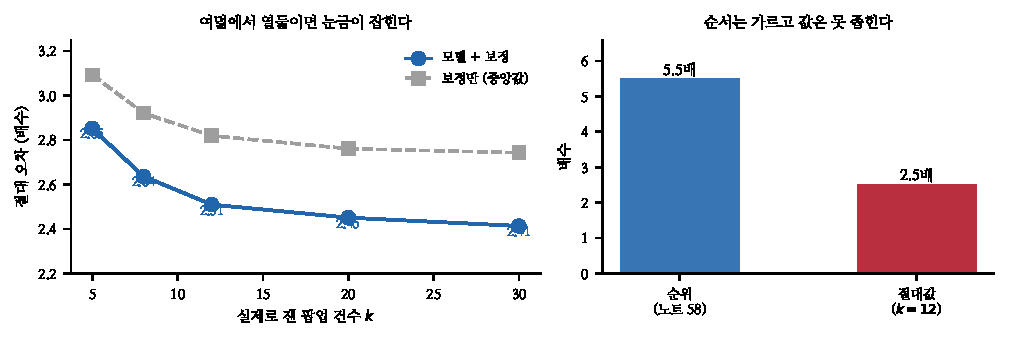
\includegraphics[width=\textwidth]{figs/calib.pdf}
\caption{왼쪽 --- 보정 건수와 절대 오차. 오른쪽 --- 순위와 절대값의 간극.}
\end{figure}

\begin{table}[t]
\centering\tsize
\caption{보정 건수별 절대 오차. 400회 무작위 분할 평균.}
\begin{tabular}{lrrr}
\toprule
$k$ & 모델$+$보정 & 중앙값만 & 배수 오차 \\
\midrule
5 & 0.4551 & 0.4903 & 2.85배 \\
8 & 0.4210 & 0.4655 & 2.64배 \\
\textbf{12} & \textbf{0.3995} & 0.4500 & \textbf{2.51배} \\
20 & 0.3892 & 0.4410 & 2.45배 \\
30 & 0.3825 & 0.4381 & 2.41배 \\
\bottomrule
\end{tabular}
\end{table}

$k=8$에서 12로 가면 0.42에서 0.40으로 줄고, 30까지 늘려도 0.38이다.
\textbf{노트 32의 ``눈금 보정에는 여덟 건이면 된다''가 여섯 도메인에서
확인된다.}

\claimx{절대 예측 오차는 열두 건을 재면 $\times\div$2.51배이고, 더 재도 크게
줄지 않는다. 모델이 중앙값 대비 줄이는 몫은 11\%다.}{보정용 표본을 층화 없이
무작위로 뽑았다. 연도나 규모로 층화하면 적은 $k$에서 더 나을 수 있다.}

\section{간극이 어디서 오나}

순위는 5.5배로 가르는데 절대 오차는 2.5배다. 모순이 아니라 서로 다른 것을 재는
것이다.

\begin{quote}\fontsize{9.5}{11.5}\selectfont
순위 상관이 $\rho$면 설명되는 분산이 $\rho^2$이고 잔차 표준편차가
$\sqrt{1-\rho^2}$배로 남는다. $\rho=+0.47$이면 22\%를 설명하고 잔차가 원래의
88\%다. \textbf{양 끝을 갈라 놓는 데는 그것으로 충분하고, 값을 좁히는 데는
턱없이 모자란다.}
\end{quote}

\begin{table}[t]
\centering\tsize
\caption{같은 모델의 두 얼굴.}
\begin{tabular}{lr}
\toprule
순위 --- 상위 20\% $\div$ 하위 20\% & 5.5배 \\
절대값 --- 예측 오차($k{=}12$) & $\times\div$2.51배 \\
\midrule
443명 예측의 실제 범위 & 약 180--1,100명 \\
\bottomrule
\end{tabular}
\end{table}

\claimx{제품 진술은 이렇게 써야 한다 --- \textbf{어느 기획을 먼저 밀지 고르는
데는 쓸 수 있고, 몇 명 올지 약속하는 데는 아직 못 쓴다.}}{절대 오차를 줄이려면
$\rho$를 올려야 하고, $\rho$를 올리는 길은 노트 33 이후 계속 대상 도메인의
측정뿐이다. 팝업 75건이 그 병목이다.}

\section{한계}

\begin{itemize}[leftmargin=1.1em,itemsep=0.15em]
\item 보정용 표본을 무작위로 뽑았다. 실무에서는 ``비슷한 기획''을 골라 잴 것이고
      그러면 더 나을 수 있다.
\item 기울기 축소의 사전값 0.45를 노트 58의 관측 $\rho$에서 가져왔다. 새 도메인에서는
      그 값을 모른다.
\item 400회 분할 평균이라 $k$가 클수록 검정 표본이 줄어 오차 추정이 불안정하다.
\item 팝업 라벨 자체의 잡음(계수 기준 · 출처 신뢰도)이 오차에 포함돼 있다.
      노트 1--8에서 걸렀지만 남은 몫을 따로 재지 않았다.
\item 이 숫자는 팝업 75건 기준이다. 표본이 늘면 $\rho$와 함께 개선될 것이다.
\end{itemize}

\section{다음}

\begin{enumerate}[leftmargin=1.3em,itemsep=0.15em]
\item 보정용 표본을 층화해서 뽑으면 적은 $k$에서 얼마나 나아지는지.
\item 웹툰 전체 수집 완료 후 전면 재측정(1,315/3,973 진행 중).
\item $\rho$를 올리는 유일한 길 --- 팝업 표본과 축.
\item 절대값이 필요 없는 쓰임을 정리한다. 순위만으로 되는 의사결정이 무엇인지.
\end{enumerate}

\vspace{0.6em}
\hrule height 0.3pt
\vspace{0.5em}
{\footnotesize
\textbf{참고문헌}\\[0.3em]
Copas, J. B. (1983). Regression, prediction and shrinkage. \emph{JRSS B},
45(3), 311--354.\\[0.15em]
Rousseeuw, P. J., Croux, C. (1993). Alternatives to the median absolute deviation.
\emph{JASA}, 88(424), 1273--1283.\\[0.15em]
Stein, C. (1956). Inadmissibility of the usual estimator for the mean of a
multivariate normal distribution. \emph{Proc. Third Berkeley Symp.}, 1, 197--206.\\[0.15em]
Spearman, C. (1904). The proof and measurement of association between two things.
\emph{American Journal of Psychology}, 15(1), 72--101.\\[0.15em]
Ben-David, S. et al. (2010). A theory of learning from different domains.
\emph{Machine Learning}, 79(1--2), 151--175.
}

\end{document}
